\documentclass[landscape]{article}
\pagenumbering{gobble}

\usepackage[a4paper]{geometry}
\usepackage[utf8]{inputenc}
\usepackage{tikz}
\usepackage[compat=1.1.0]{tikz-feynman}
\usepackage{graphicx}

\begin{document}
\centering
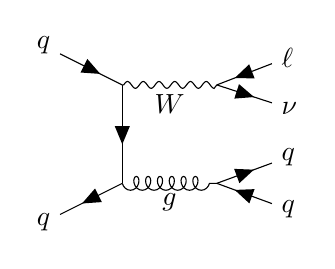
\begin{tikzpicture}
  \begin{feynman}
    % initial state particles
    \vertex (i1) {\(q\)};
    \vertex [below=2.25cm of i1] (i2) {\(q\)};

    % vertices
    \vertex [below right=0.5cm and 1cm of i1] (a1);
    \vertex [above right=0.5cm and 1cm of i2] (a2);
    \vertex [right=1.2cm of a1] (b1);
    \vertex [right=1.2cm of a2] (b2);

    % final state particles
    \vertex [above right=0.1cm and 0.7cm of b1] (f1) {\(\ell\)};
    \vertex [below right=0.1cm and 0.7cm of b1] (f2) {\(\nu\)};
    \vertex [above right=0.1cm and 0.7cm of b2] (f3) {$q$};
    \vertex [below right=0.1cm and 0.7cm of b2] (f4) {$q$};

    \diagram* {
      (i1) -- [fermion] (a1) -- [fermion] (a2)
        -- [fermion] (i2),

      (a1) -- [boson, edge label'=\(W\)] (b1),
      (a2) -- [gluon, edge label'=\(g\)] (b2),

      (f1) -- [fermion] (b1)
        -- [fermion] (f2),

      (f4) -- [fermion] (b2)
        -- [fermion] (f3),
    };


  \end{feynman}
\end{tikzpicture}%
\end{document}
